\providecommand{\Mod}{\mathbb{M}od}
\providecommand{\Fun}{\operatorname{Fun}}
\providecommand{\HomA}{\mathrm{Hom}_{A}}
\providecommand{\HomB}{\mathrm{Hom}_{B}}
\providecommand{\Hom}{\mathrm{Hom}}

\section{虚拟装备的双等价}\label{sec:biequivalence-of-virtual-equipments}

在本节中，我们将证明：一个\trCosmologicalBiequivalence{}
$F\colon\mathcal{K}\Rightarrow\mathcal{L}$ 诱导诸虚拟装备之间的一个%
\emph{\trBiequivalence}
$F\colon\Mod(\mathcal{K})\Rightarrow\Mod(\mathcal{L})$。随后我们将解释这一结果
的含义：诸\trInfinityCategory{}的范畴论会被任何这种形式的「\trChangeOfModel{}」%
\trFunctor{}保持、反射并创造。

「诸\trInfinityCategory{}的理论是\trModelIndependent{}」这一主张无疑应当涵盖如下这样的
断言：
\begin{itemize}
\item 诸\trInfinityCategory{}之间的一个\trFunctor{}在一个特定的模型中拥有一个%
\trLeftAdjoint，当且仅当它在每一个模型中都拥有一个\trLeftAdjoint。
\item 一个以\trInfinityCategory{}为取值的\trDiagram{}在某个模型中拥有一个%
\trLimit，当且仅当它在每一个模型中都拥有一个\trLimit。
\end{itemize}

在我们的设定中，诸如 \eqref{eq:four-model-cosmoi} 那样的诸\trChangeOfModel{}%
\trFunctor{}定义诸\trCosmologicalBiequivalence，或由之构成的之字形链。沿着这些
思路，10.3 节中发展出了一种证明诸\trInfinityCategory{}的基本范畴论之%
\trModelIndependence{}的特设方法，在那里我们观察到：在双等价的诸%
\trInfinityCosmos{}之间，∞-范畴性数据与性质的特设翻译如果需要的话，可以相对
机械地、以极其烦冗的细节给出。

对\trModelIndependence{}的一种更为系统化的进路，会利用诸\trInfinityCategory{}的
形式范畴论的那个最为全面的框架，即模的\trVirtualEquipment。我们简要回顾其本质
特征。请回忆第 8 章：一个\trInfinityCosmos{} $\mathcal{K}$ 中的模的%
\textbf{\trVirtualDoubleCategory} $\Mod(\mathcal{K})$ 由下列诸项构成：

\begin{itemize}
\item 一个由\textbf{对象}与\textbf{竖直箭头}构成的\trCategory，此处即诸%
\trInfinityCategory{}与诸\trInfinityFunctor，竖直地描绘；
\item 对任意一对对象 $A$、$B$，一个由\textbf{水平箭头} $A\xrightarrow{E}B$ 组成
的汇集，此处即从 $A$ 到 $B$ 的诸\trModule{} $(q,p)\colon E\twoheadrightarrow A\times B$；
\item 诸\textbf{\trCell}，其边界描绘如下
\begin{center}
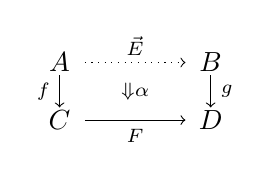
\begin{tikzpicture}[x=1.3em,y=1.3em]
  \node at (0,1.6) {$A$};
  \node at (4.2,1.6) {$B$};
  \draw[->,dotted] (0.7,1.6) -- (3.5,1.6);
  \node at (2.1,2.05) {$\scriptstyle\vec{E}$};
  \draw[->] (0,1.25) -- (0,0.35);
  \node at (-0.45,0.8) {$\scriptstyle f$};
  \draw[->] (4.2,1.25) -- (4.2,0.35);
  \node at (4.65,0.8) {$\scriptstyle g$};
  \node at (2.1,0.8) {$\scriptstyle\Downarrow\alpha$};
  \node at (0,0) {$C$};
  \node at (4.2,0) {$D$};
  \draw[->] (0.7,0) -- (3.5,0);
  \node at (2.1,-0.45) {$\scriptstyle F$};
\end{tikzpicture}
\end{center}
其中 $\vec{E}$ 是从 $A$ 到 $B$ 的一个模的相容序列
$E_{1}\divideontimes\cdots\divideontimes E_{n}$ 之缩写，在 $A=B$ 的情形下它可以
为空。此处，具有所示边界的一支\trCell{}是\trFunctorSpace{}
$\Fun_{f\times g}(\vec{E},F)$ 中对象的一个\trIsomorphism{}类，该空间由从双侧%
\trFibration{} $A\twoheadleftarrow\vec{E}\twoheadrightarrow B$ 到
$C\twoheadleftarrow F\twoheadrightarrow D$ 的、位于 $f\times g$ 之上的那些映射
构成；
\item 一支\textbf{复合}\trCell，对任何如下构型
\begin{center}
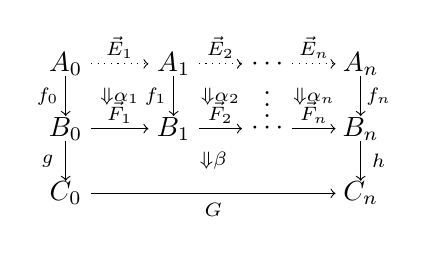
\begin{tikzpicture}[x=1.3em,y=1.3em]
  \node at (0,3.2)   {$A_{0}$};
  \node at (3.0,3.2) {$A_{1}$};
  \node at (5.6,3.2) {$\cdots$};
  \node at (8.2,3.2) {$A_{n}$};
  \draw[->,dotted] (0.7,3.2) -- (2.3,3.2);
  \node at (1.5,3.65) {$\scriptstyle\vec{E}_{1}$};
  \draw[->,dotted] (3.7,3.2) -- (4.9,3.2);
  \node at (4.3,3.65) {$\scriptstyle\vec{E}_{2}$};
  \draw[->,dotted] (6.3,3.2) -- (7.5,3.2);
  \node at (6.9,3.65) {$\scriptstyle\vec{E}_{n}$};
  \draw[->] (0,2.85) -- (0,1.75);
  \node at (-0.5,2.3) {$\scriptstyle f_{0}$};
  \draw[->] (3.0,2.85) -- (3.0,1.75);
  \node at (2.5,2.3) {$\scriptstyle f_{1}$};
  \node at (5.6,2.3) {$\vdots$};
  \draw[->] (8.2,2.85) -- (8.2,1.75);
  \node at (8.7,2.3) {$\scriptstyle f_{n}$};
  \node at (1.5,2.3) {$\scriptstyle\Downarrow\alpha_{1}$};
  \node at (4.3,2.3) {$\scriptstyle\Downarrow\alpha_{2}$};
  \node at (6.9,2.3) {$\scriptstyle\Downarrow\alpha_{n}$};
  \node at (0,1.4)   {$B_{0}$};
  \node at (3.0,1.4) {$B_{1}$};
  \node at (5.6,1.4) {$\cdots$};
  \node at (8.2,1.4) {$B_{n}$};
  \draw[->] (0.7,1.4) -- (2.3,1.4);
  \node at (1.5,1.85) {$\scriptstyle\vec{F}_{1}$};
  \draw[->] (3.7,1.4) -- (4.9,1.4);
  \node at (4.3,1.85) {$\scriptstyle\vec{F}_{2}$};
  \draw[->] (6.3,1.4) -- (7.5,1.4);
  \node at (6.9,1.85) {$\scriptstyle\vec{F}_{n}$};
  \draw[->] (0,1.05) -- (0,-0.05);
  \node at (-0.5,0.5) {$\scriptstyle g$};
  \draw[->] (8.2,1.05) -- (8.2,-0.05);
  \node at (8.7,0.5) {$\scriptstyle h$};
  \node at (4.1,0.5) {$\scriptstyle\Downarrow\beta$};
  \node at (0,-0.4)  {$C_{0}$};
  \node at (8.2,-0.4){$C_{n}$};
  \draw[->] (0.7,-0.4) -- (7.5,-0.4);
  \node at (4.1,-0.85) {$\scriptstyle G$};
\end{tikzpicture}
\end{center}
它由先拉回、随后复合诸跨度之映射的\trFiberedIsomorphism{}类而定义；
\item 一支\textbf{恒同}\trCell，对每一支水平箭头
\begin{center}
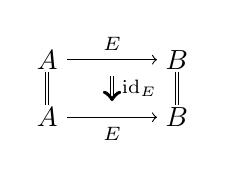
\begin{tikzpicture}[x=1.3em,y=1.3em]
  \node at (0,1.6) {$A$};
  \node at (3.6,1.6) {$B$};
  \node at (0,0) {$A$};
  \node at (3.6,0) {$B$};
  \draw[->] (0.55,1.6) -- (3.05,1.6);
  \node at (1.8,2.05) {$\scriptstyle E$};
  \draw[double,double distance=0.6pt] (0,1.25) -- (0,0.35);
  \draw[double,double distance=0.6pt] (3.6,1.25) -- (3.6,0.35);
  \draw[double,->] (1.8,1.15) -- node[right]{$\scriptstyle\mathrm{id}_{E}$} (1.8,0.45);
  \draw[->] (0.55,0) -- (3.05,0);
  \node at (1.8,-0.45) {$\scriptstyle E$};
\end{tikzpicture}
\end{center}
\end{itemize}
使得诸\trCell{}的复合在通常的多范畴意义下是严格结合且幺的。

\begin{lemma}\label{lem:cosmological-functor-induces-vdc-functor}
一个\trCosmologicalFunctor{}诱导诸\trVirtualDoubleCategory{}之间的一个%
\trFunctor，并保持全部结构。
\end{lemma}

\begin{proof}
在\cref{cor:virtual-double-category-of-modules}中，模的\trVirtualDoubleCategory{}%
里的诸范畴论结构承袭自双侧等价纤维化的\trDoubleCategory。我们可以沿类似的路线来
理解一个\trCosmologicalFunctor{} $F\colon\mathcal{K}\to\mathcal{L}$ 在模的%
\trVirtualDoubleCategory{}上的作用。

如\cref{ex:cosmos-of-two-sided-isofibrations}所述，双侧等价纤维化的非幺%
\trDoubleCategory{}可以理解为诸\trInfinityCosmos{}与诸\trCosmologicalFunctor{}的
一个「非幺内范畴」（见定义 B.1.8）的商
\begin{equation*}
\mathcal{K}^{\times}\times_{\mathcal{K}}\mathcal{K}^{\times}
\xrightarrow{\ \circ\ }
\mathcal{K}^{\times}
\;\overset{\text{l-cod}}{\underset{\text{r-cod}}{\rightrightarrows}}\;
\mathcal{K}
\end{equation*}
其中 $\mathcal{K}^{\times}$ 是双侧等价纤维化的\trInfinityCosmos，而
$\text{l-cod}$ 与 $\text{r-cod}\colon\mathcal{K}^{\times}\to\mathcal{K}$ 是把一
条双侧等价纤维化
$A\overset{q}{\twoheadleftarrow}E\overset{p}{\twoheadrightarrow}B$ 送到该\trSpan{}%
的基\trInfinityCategory{} $A$ 与 $B$ 的左、右余定义域\trFunctor。注意这些%
\trFunctor{}合起来定义一个 Grothendieck \trFibration{}
$\mathrm{cod}\colon\mathcal{K}^{\times}\to\mathcal{K}\times\mathcal{K}$。\trPullback
\begin{center}
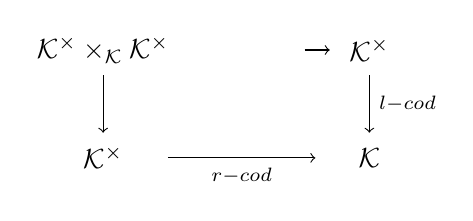
\begin{tikzpicture}[x=1.3em,y=1.3em]
  \node (a) at (0,1.5)   {$\mathcal{K}^{\times}\times_{\mathcal{K}}\mathcal{K}^{\times}$};
  \node (b) at (7.4,1.5) {$\mathcal{K}^{\times}$};
  \node (c) at (0,-1.5)  {$\mathcal{K}^{\times}$};
  \node (d) at (7.4,-1.5){$\mathcal{K}$};
  \draw[->] (5.6,1.5) -- (6.3,1.5);
  \draw[->] (0,0.8) -- (0,-0.8);
  \draw[->] (7.4,0.8) -- node[right]{$\scriptstyle\text{l-cod}$} (7.4,-0.8);
  \draw[->] (1.8,-1.5) -- node[below]{$\scriptstyle\text{r-cod}$} (5.9,-1.5);
  \node at (1.9,0.7) {$\scriptstyle\lrcorner$};
\end{tikzpicture}
\end{center}
是一个\trInfinityCosmos{}（见练习 6.1.iii），即水平可复合的一对双侧等价纤维化
$A\overset{q}{\twoheadleftarrow}E\overset{p}{\twoheadrightarrow}B\overset{r}{\twoheadleftarrow}F\overset{s}{\twoheadrightarrow}C$
之\trInfinityCosmos。复合\trFunctor{}
$\circ\colon\mathcal{K}^{\times}\times_{\mathcal{K}}\mathcal{K}^{\times}\to\mathcal{K}^{\times}$
把一对水平可复合的双侧等价纤维化送到一条选定的复合\trSpan，它仅在单纯自然同构的
意义下结合，这正是双侧等价纤维化的\trDoubleCategory{}中水平复合之「伪性」的
缘由。（非幺伪）双侧等价纤维化的\trDoubleCategory{}可以理解为这一结构的一个商：
把\trInfinityCosmos{} $\mathcal{K}$ 换成其底\trCategory，并把
$\mathrm{cod}\colon\mathcal{K}^{\times}\to\mathcal{K}\times\mathcal{K}$ 的诸纤维
换成诸商 1-范畴——后者拥有相同的对象，但其 hom-集被定义为切片\trFunctorSpace{}%
中诸顶点的\trIsomorphism{}类。

现在，任何\trCosmologicalFunctor{} $F\colon\mathcal{K}\to\mathcal{L}$ 都诱导诸%
\trCosmologicalFunctor
\begin{center}
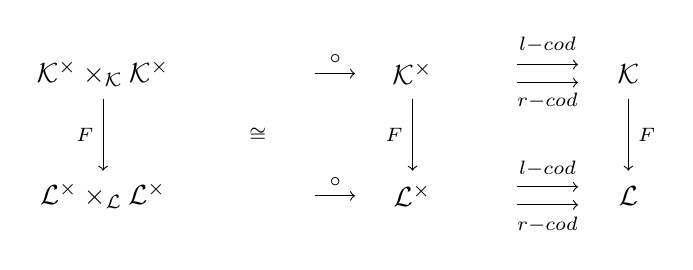
\begin{tikzpicture}[x=1.3em,y=1.3em]
  \node (a) at (0,1.7)    {$\mathcal{K}^{\times}\times_{\mathcal{K}}\mathcal{K}^{\times}$};
  \node (b) at (8.6,1.7)  {$\mathcal{K}^{\times}$};
  \node (c) at (14.6,1.7) {$\mathcal{K}$};
  \node (d) at (0,-1.7)   {$\mathcal{L}^{\times}\times_{\mathcal{L}}\mathcal{L}^{\times}$};
  \node (e) at (8.6,-1.7) {$\mathcal{L}^{\times}$};
  \node (f) at (14.6,-1.7){$\mathcal{L}$};
  \draw[->] (5.9,1.7) -- node[above]{$\scriptstyle\circ$} (7.0,1.7);
  \draw[->] (11.5,1.95) -- (13.2,1.95);
  \draw[->] (11.5,1.45) -- (13.2,1.45);
  \node at (12.35,2.5) {$\scriptstyle\text{l-cod}$};
  \node at (12.35,0.95) {$\scriptstyle\text{r-cod}$};
  \draw[->] (5.9,-1.7) -- node[above]{$\scriptstyle\circ$} (7.0,-1.7);
  \draw[->] (11.5,-1.45) -- (13.2,-1.45);
  \draw[->] (11.5,-1.95) -- (13.2,-1.95);
  \node at (12.35,-0.95) {$\scriptstyle\text{l-cod}$};
  \node at (12.35,-2.5) {$\scriptstyle\text{r-cod}$};
  \draw[->] (0,1.0) -- node[left]{$\scriptstyle F$} (0,-1.0);
  \draw[->] (8.6,1.0) -- node[left]{$\scriptstyle F$} (8.6,-1.0);
  \draw[->] (14.6,1.0) -- node[right]{$\scriptstyle F$} (14.6,-1.0);
  \node at (4.3,0) {$\scriptstyle\cong$};
\end{tikzpicture}
\end{center}
它们与诸余定义域\trFunctor{}严格交换，而与复合\trFunctor{}至多差一个同构。于是，
一个\trCosmologicalFunctor{}诱导双侧等价纤维化的诸\trDoubleCategory{}之间的一个
双函子，后者严格保持\trFunctor{}与方块的竖直复合，并在相干自然同构的意义下保持%
\trSpan{}与方块的水平复合。

由此得出：一个\trCosmologicalFunctor{}
$F\colon\mathcal{K}\to\mathcal{L}$ 诱导模的诸\trVirtualDoubleCategory{}之间的一个%
\trFunctor{} $F\colon\Mod(\mathcal{K})\to\Mod(\mathcal{L})$，它严格保持全部结构，
因为模映射的多范畴式复合派生自双侧等价纤维化的\trDoubleCategory{}中严格定义
的竖直复合。
\end{proof}

就其作为形式范畴论舞台的效用而言，至关重要的事实是：
模的\trVirtualDoubleCategory{}是一个\trVirtualEquipment，意谓它满足如下两条进
一步的性质：

\begin{enumerate}[label=(\roman*)]
\item 对任何一支\trModule{}与一对\trFunctor——如下左图所示——都存在一个%
\textbf{限制}\trModule{}与一支\textbf{笛卡尔的}\trCell，如下右图所示
\begin{center}
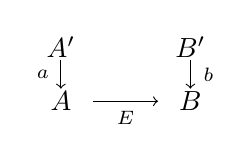
\begin{tikzpicture}[x=1.3em,y=1.3em]
  \node at (0,1.5) {$A'$};
  \node at (3.6,1.5) {$B'$};
  \node at (0,0) {$A$};
  \node at (3.6,0) {$B$};
  \draw[->] (0,1.15) -- (0,0.35);
  \node at (-0.5,0.75) {$\scriptstyle a$};
  \draw[->] (3.6,1.15) -- (3.6,0.35);
  \node at (4.1,0.75) {$\scriptstyle b$};
  \draw[->] (0.9,0) -- (2.7,0);
  \node at (1.8,-0.45) {$\scriptstyle E$};
\end{tikzpicture}
\qquad$\rightsquigarrow$\qquad
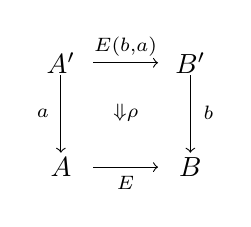
\begin{tikzpicture}[x=1.3em,y=1.3em]
  \node at (0,2.9) {$A'$};
  \node at (3.6,2.9) {$B'$};
  \node at (0,0) {$A$};
  \node at (3.6,0) {$B$};
  \draw[->] (0.9,2.9) -- (2.7,2.9);
  \node at (1.8,3.35) {$\scriptstyle E(b,a)$};
  \draw[->] (0,2.55) -- (0,0.4);
  \node at (-0.5,1.5) {$\scriptstyle a$};
  \draw[->] (3.6,2.55) -- (3.6,0.4);
  \node at (4.1,1.5) {$\scriptstyle b$};
  \node at (1.8,1.5) {$\scriptstyle\Downarrow\rho$};
  \draw[->] (0.9,0) -- (2.7,0);
  \node at (1.8,-0.45) {$\scriptstyle E$};
\end{tikzpicture}
\end{center}
并由如下\trUniversalProperty{}刻画：任何如下左图所示的\trCell{}都经由 $\rho$
唯一地分解，如下右图所示：
\begin{center}
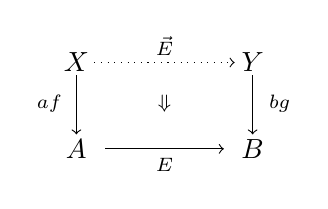
\begin{tikzpicture}[x=1.3em,y=1.3em]
  \node at (0,3) {$X$};
  \node at (4.9,3) {$Y$};
  \draw[->,dotted] (0.5,3) -- (4.4,3);
  \node at (2.45,3.45) {$\scriptstyle\vec{E}$};
  \draw[->] (0,2.65) -- (0,1.0);
  \node at (-0.75,1.85) {$\scriptstyle af$};
  \draw[->] (4.9,2.65) -- (4.9,1.0);
  \node at (5.65,1.85) {$\scriptstyle bg$};
  \node at (2.45,1.85) {$\scriptstyle\Downarrow$};
  \node at (0,0.6) {$A$};
  \node at (4.9,0.6) {$B$};
  \draw[->] (0.8,0.6) -- (4.1,0.6);
  \node at (2.45,0.15) {$\scriptstyle E$};
\end{tikzpicture}
\qquad $=$ \qquad
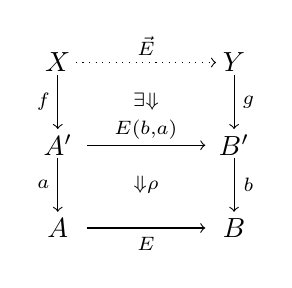
\begin{tikzpicture}[x=1.3em,y=1.3em]
  \node at (0,4.6) {$X$};
  \node at (4.9,4.6) {$Y$};
  \draw[->,dotted] (0.5,4.6) -- (4.4,4.6);
  \node at (2.45,5.05) {$\scriptstyle\vec{E}$};
  \draw[->] (0,4.25) -- (0,2.75);
  \node at (-0.4,3.5) {$\scriptstyle f$};
  \node at (2.45,3.5) {$\scriptstyle\exists\Downarrow$};
  \draw[->] (4.9,4.25) -- (4.9,2.75);
  \node at (5.3,3.5) {$\scriptstyle g$};
  \node at (0,2.3) {$A'$};
  \node at (4.9,2.3) {$B'$};
  \draw[->] (0.8,2.3) -- (4.1,2.3);
  \node at (2.45,2.72) {$\scriptstyle E(b,a)$};
  \draw[->] (0,1.95) -- (0,0.45);
  \node at (-0.4,1.2) {$\scriptstyle a$};
  \draw[->] (4.9,1.95) -- (4.9,0.45);
  \node at (5.3,1.2) {$\scriptstyle b$};
  \node at (2.45,1.2) {$\scriptstyle\Downarrow\rho$};
  \node at (0,0) {$A$};
  \node at (4.9,0) {$B$};
  \draw[->] (0.8,0) -- (4.1,0);
  \node at (2.45,-0.45) {$\scriptstyle E$};
\end{tikzpicture}
\end{center}
限制\trModule{}由把一支\trModule{} $A\xrightarrow{E}B$ 沿\trFunctor{}
$a\colon A'\to A$ 与 $b\colon B'\to B$ 作\trPullback{}而定义。定义
$E(b,a)$ 的那个单纯\trPullback{}诱导\trFunctorSpace{}之间的一个\trEquivalence
\begin{equation*}
\Fun_{af\times bg}(E_{1}\divideontimes\cdots\divideontimes E_{n},\,E)
\simeq
\Fun_{f\times g}(E_{1}\divideontimes\cdots\divideontimes E_{n},\,E(b,a)),
\end{equation*}
它给出这一\trUniversalProperty{}（见\cref{prop:restriction}）。
\item 每个对象 $A$ 都拥有一个\textbf{单位}\trModule，配备有一支零元\textbf{余笛卡尔的}%
\trCell
\begin{center}
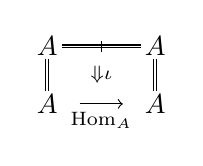
\begin{tikzpicture}[x=1.3em,y=1.3em]
  \node at (0,1.6) {$A$};
  \node at (3.0,1.6) {$A$};
  \node at (0,0) {$A$};
  \node at (3.0,0) {$A$};
  \draw[double,double distance=0.6pt] (0.4,1.6) -- (2.6,1.6);
  \draw (1.5,1.75) -- (1.5,1.45);
  \draw[double,double distance=0.6pt] (0,1.25) -- (0,0.35);
  \draw[double,double distance=0.6pt] (3.0,1.25) -- (3.0,0.35);
  \node at (1.5,0.8) {$\scriptstyle\Downarrow\iota$};
  \draw[->] (0.9,0) -- (2.1,0);
  \node at (1.5,-0.45) {$\scriptstyle\HomA$};
\end{tikzpicture}
\end{center}
满足如下\trUniversalProperty{}：模的\trVirtualDoubleCategory{}中任何水平源包含
对象 $A$ 的\trCell——如下左图所示——都经由 $\iota$ 唯一地分解，如下右图所示：
\begin{center}
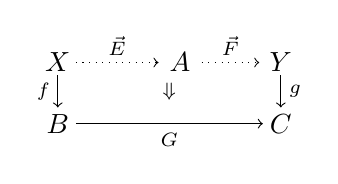
\begin{tikzpicture}[x=1.3em,y=1.3em]
  \node at (0,1.7) {$X$};
  \node at (3.4,1.7) {$A$};
  \node at (6.2,1.7) {$Y$};
  \draw[->,dotted] (0.5,1.7) -- (2.8,1.7);
  \node at (1.65,2.15) {$\scriptstyle\vec{E}$};
  \draw[->,dotted] (4.0,1.7) -- (5.6,1.7);
  \node at (4.8,2.15) {$\scriptstyle\vec{F}$};
  \draw[->] (0,1.35) -- (0,0.45);
  \node at (-0.4,0.9) {$\scriptstyle f$};
  \draw[->] (6.2,1.35) -- (6.2,0.45);
  \node at (6.6,0.9) {$\scriptstyle g$};
  \node at (3.1,0.9) {$\scriptstyle\Downarrow$};
  \node at (0,0) {$B$};
  \node at (6.2,0) {$C$};
  \draw[->] (0.5,0) -- (5.7,0);
  \node at (3.1,-0.45) {$\scriptstyle G$};
\end{tikzpicture}
\qquad $=$ \qquad
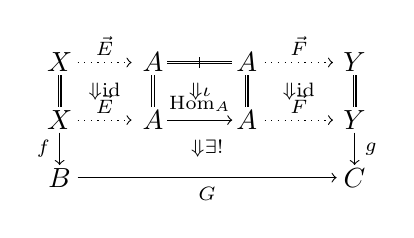
\begin{tikzpicture}[x=1.3em,y=1.3em]
  \node at (0,3.4) {$X$};
  \node at (2.6,3.4) {$A$};
  \node at (5.2,3.4) {$A$};
  \node at (8.2,3.4) {$Y$};
  \draw[->,dotted] (0.5,3.4) -- (2.0,3.4);
  \node at (1.25,3.85) {$\scriptstyle\vec{E}$};
  \draw[double,double distance=0.6pt] (3.0,3.4) -- (4.8,3.4);
  \draw (3.9,3.55) -- (3.9,3.25);
  \draw[->,dotted] (5.7,3.4) -- (7.6,3.4);
  \node at (6.65,3.85) {$\scriptstyle\vec{F}$};
  \draw[double,double distance=0.6pt] (0,3.05) -- (0,2.15);
  \draw[double,double distance=0.6pt] (2.6,3.05) -- (2.6,2.15);
  \draw[double,double distance=0.6pt] (5.2,3.05) -- (5.2,2.15);
  \draw[double,double distance=0.6pt] (8.2,3.05) -- (8.2,2.15);
  \node at (1.25,2.6) {$\scriptstyle\Downarrow\mathrm{id}$};
  \node at (3.9,2.6) {$\scriptstyle\Downarrow\iota$};
  \node at (6.65,2.6) {$\scriptstyle\Downarrow\mathrm{id}$};
  \node at (0,1.8) {$X$};
  \node at (2.6,1.8) {$A$};
  \node at (5.2,1.8) {$A$};
  \node at (8.2,1.8) {$Y$};
  \draw[->,dotted] (0.5,1.8) -- (2.0,1.8);
  \node at (1.25,2.25) {$\scriptstyle\vec{E}$};
  \draw[->] (3.0,1.8) -- (4.8,1.8);
  \node at (3.9,2.25) {$\scriptstyle\HomA$};
  \draw[->,dotted] (5.7,1.8) -- (7.6,1.8);
  \node at (6.65,2.25) {$\scriptstyle\vec{F}$};
  \draw[->] (0,1.45) -- (0,0.55);
  \node at (-0.45,1.0) {$\scriptstyle f$};
  \draw[->] (8.2,1.45) -- (8.2,0.55);
  \node at (8.65,1.0) {$\scriptstyle g$};
  \node at (4.1,1.0) {$\scriptstyle\Downarrow\exists!$};
  \node at (0,0.2) {$B$};
  \node at (8.2,0.2) {$C$};
  \draw[->] (0.5,0.2) -- (7.7,0.2);
  \node at (4.1,-0.25) {$\scriptstyle G$};
\end{tikzpicture}
\end{center}
单位\trModule{}即箭头∞-范畴，当把它视为一个从 $A$ 到 $A$ 的\trModule{}时，记作
$A\xrightarrow{\HomA}A$。这一\trUniversalProperty{}由\trYonedaLemma{}得出（见
\cref{prop:units}）。
\end{enumerate}

\cref{lem:cosmological-functor-induces-vdc-functor}扩张到诸模的虚拟装备：

\begin{proposition}\label{prop:cosmological-functor-induces-ve-functor}
一个\trCosmologicalFunctor{}
$F\colon\mathcal{K}\to\mathcal{L}$ 诱导诸\trVirtualEquipment{}之间的%
\trFunctor{}
$F\colon\Mod(\mathcal{K})\to\Mod(\mathcal{L})$，并保持全部结构。
\end{proposition}

\begin{proof}
鉴于\cref{lem:cosmological-functor-induces-vdc-functor}，尚需考虑的只是单位与
限制的\trModule{}及\trCell。由\cref{prop:units}与\cref{prop:restriction}的证明中
所给的构造，立见这些皆为诸\trCosmologicalFunctor{}所保持：
\begin{center}
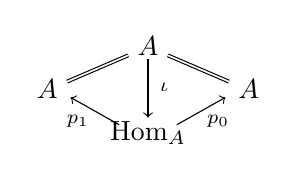
\begin{tikzpicture}[x=1.3em,y=1.3em]
  \node at (0,2.4) {$A$};
  \node at (-2.8,1.2) {$A$};
  \node at (2.8,1.2) {$A$};
  \node at (0,0) {$\HomA$};
  \draw[double,double distance=0.6pt] (-0.55,2.15) -- (-2.25,1.42);
  \draw[double,double distance=0.6pt] (0.55,2.15) -- (2.25,1.42);
  \draw[->] (0,2.05) -- (0,0.42);
  \node at (0.45,1.25) {$\scriptstyle\iota$};
  \draw[->] (-0.8,0.22) -- (-2.15,0.98);
  \node at (-1.95,0.32) {$\scriptstyle p_{1}$};
  \draw[->] (0.8,0.22) -- (2.15,0.98);
  \node at (1.95,0.32) {$\scriptstyle p_{0}$};
\end{tikzpicture}
\qquad
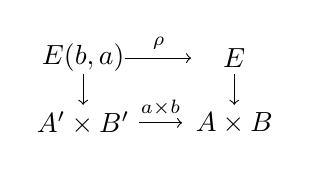
\begin{tikzpicture}[x=1.3em,y=1.3em]
  \node at (0,1.8) {$E(b,a)$};
  \node at (4.2,1.8) {$E$};
  \node at (0,0) {$A'\times B'$};
  \node at (4.2,0) {$A\times B$};
  \draw[->] (1.15,1.8) -- (3.0,1.8);
  \node at (2.1,2.22) {$\scriptstyle\rho$};
  \draw[->] (0,1.35) -- (0,0.5);
  \draw[->] (4.2,1.35) -- (4.2,0.5);
  \draw[->] (1.55,0) -- (2.75,0);
  \node at (2.15,0.42) {$\scriptstyle a\times b$};
  \node at (3.55,1.3) {$\scriptstyle\lrcorner$};
\end{tikzpicture}
\end{center}
\end{proof}

\trHomotopyTwoCategory{} $\mathfrak{h}\mathcal{K}$ 中的诸\trFunctor{}与诸%
\trNaturalTransformation{}以三种方式嵌入虚拟装备 $\Mod(\mathcal{K})$ 之中。一个%
\trFunctor{} $f\colon A\to B$ 既被表示为一支竖直箭头，也被表示为那对水平的%
\trModule{} $A\xrightarrow{\HomB(B,f)}B$ 与
$B\xrightarrow{\HomB(f,B)}A$，它们以一种适宜于\trVirtualDoubleCategory{}的意义
表现得如同伴随：\trModule{} $A\xrightarrow{\HomB(B,f)}B$ 定义竖直箭头
$f\colon A\to B$ 的一个\emph{\trCompanion}，而\trModule{}
$B\xrightarrow{\HomB(f,B)}A$ 则定义其一个\emph{\trConjoint}（见
\cref{prop:representable-restriction-application}、\cref{thm:spider-lemma}与
\cref{cor:represented-composites}）。借助\cref{prop:two-cell-bijections}，这些
嵌入扩张到诸\trNaturalTransformation{}上：对任何平行的\trFunctor{}对，在同伦
2-范畴
\begin{center}
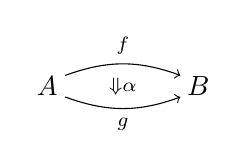
\begin{tikzpicture}[x=1.3em,y=1.3em]
  \node (a) at (0,0) {$A$};
  \node (b) at (4.2,0) {$B$};
  \draw[->] (0.5,0.3) to[bend left=20] node[above,pos=0.5]{$\scriptstyle f$} (3.7,0.3);
  \draw[->] (0.5,-0.3) to[bend right=20] node[below,pos=0.5]{$\scriptstyle g$} (3.7,-0.3);
  \node at (2.1,0) {$\scriptstyle\Downarrow\alpha$};
\end{tikzpicture}
\end{center}
中的诸\trNaturalTransformation{}与模的\trVirtualEquipment{}中的诸\trCell{}之间
存在自然双射：
\begin{center}
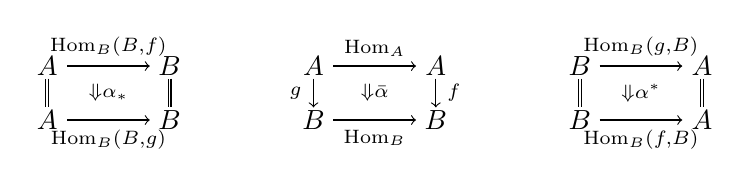
\begin{tikzpicture}[x=1.3em,y=1.3em]
  \node at (0,1.5) {$A$};
  \node at (3.4,1.5) {$B$};
  \node at (0,0) {$A$};
  \node at (3.4,0) {$B$};
  \draw[->] (0.55,1.5) -- node[above]{$\scriptstyle\HomB(B,f)$} (2.85,1.5);
  \draw[->] (0.55,0) -- node[below]{$\scriptstyle\HomB(B,g)$} (2.85,0);
  \draw[double,double distance=0.6pt] (0,1.15) -- (0,0.35);
  \draw[double,double distance=0.6pt] (3.4,1.15) -- (3.4,0.35);
  \node at (1.7,0.75) {$\scriptstyle\Downarrow\alpha_{*}$};
  \node at (5.4,0.75) {$\scriptstyle\rightsquigarrow$};
  \begin{scope}[shift={(7.4,0)}]
  \node at (0,1.5) {$A$};
  \node at (3.4,1.5) {$A$};
  \node at (0,0) {$B$};
  \node at (3.4,0) {$B$};
  \draw[->] (0.55,1.5) -- node[above]{$\scriptstyle\HomA$} (2.85,1.5);
  \draw[->] (0.55,0) -- node[below]{$\scriptstyle\HomB$} (2.85,0);
  \draw[->] (0,1.15) -- (0,0.35);
  \node at (-0.5,0.75) {$\scriptstyle g$};
  \draw[->] (3.4,1.15) -- (3.4,0.35);
  \node at (3.9,0.75) {$\scriptstyle f$};
  \node at (1.7,0.75) {$\scriptstyle\Downarrow\bar{\alpha}$};
  \end{scope}
  \node at (12.8,0.75) {$\scriptstyle\rightsquigarrow$};
  \begin{scope}[shift={(14.8,0)}]
  \node at (0,1.5) {$B$};
  \node at (3.4,1.5) {$A$};
  \node at (0,0) {$B$};
  \node at (3.4,0) {$A$};
  \draw[->] (0.55,1.5) -- node[above]{$\scriptstyle\HomB(g,B)$} (2.85,1.5);
  \draw[->] (0.55,0) -- node[below]{$\scriptstyle\HomB(f,B)$} (2.85,0);
  \draw[double,double distance=0.6pt] (0,1.15) -- (0,0.35);
  \draw[double,double distance=0.6pt] (3.4,1.15) -- (3.4,0.35);
  \node at (1.7,0.75) {$\scriptstyle\Downarrow\alpha^{*}$};
  \end{scope}
\end{tikzpicture}
\end{center}

正如\cref{def:covariant-contravariant-embeddings}中所评述的，作为这些结果的一
个推论，存在三个从\trHomotopyTwoCategory{} $\mathfrak{h}\mathcal{K}$ 到虚拟装备
$\Mod(\mathcal{K})$ 的\trLocallyFullyFaithful\trHomomorphism。命题 8.3.18 所描述的那个%
\emph{竖直嵌入}（vertical embedding）把 $\mathfrak{h}\mathcal{K}$ 的诸\trFunctor{}%
送到竖直箭头，并把诸 2-\trCell{}送到源与靶由单位\trModule{}给出的一元\trCell。
另外两个分别是\emph{协变嵌入}与\emph{逆变嵌入}——它们把同伦 2-范畴嵌入到
$\Mod(\mathcal{K})$ 的那个仅由竖直边界皆为恒同的一元\trCell{}构成的子结构%
\footnote{这一子结构十分接近一个\trBicategory，其中一元\trCell{}的水平复合如定义
8.3.16 那样构造，只是诸\trModule{}的相容序列并不总是拥有一个水平复合。}之中。
协变嵌入像中的诸\trModule{}是诸右可表示模，而逆变嵌入像中的诸\trModule{}则是诸
左可表示模。我们把它留给读者验证：

\begin{lemma}\label{lem:vdc-functor-commutes-with-embeddings}
由一个\trCosmologicalFunctor{}
$F\colon\mathcal{K}\to\mathcal{L}$ 所诱导的诸\trVirtualEquipment{}之间的%
\trFunctor{}
$F\colon\Mod(\mathcal{K})\to\Mod(\mathcal{L})$ 与协变嵌入、逆变嵌入及竖直嵌入相
交换。
\end{lemma}

\begin{proof}
\cref{ex:prove-embeddings-commute}。
\end{proof}

第 9 章的主题可以这样概括：一个\trInfinityCosmos{}中的模的\trVirtualEquipment{}%
是发展诸\trInfinityCategory{}的范畴论的一个稳健舞台。一方面，它包含该%
\trInfinityCosmos{}的\trHomotopyTwoCategory——第一部分中的大多数结果正是以此为
舞台的。它也是研究那些在\trHomotopyTwoCategory{}中颇为难于表述的∞-范畴性质的
一个十分自然的家园。例如，逗号∞-范畴的弱 2-泛性质现在由\cref{lem:comma-module-maps-bijection}
中的一个双射所编码：虚拟装备中余定义域为\trCommaModule{}的诸\trCell{}，与%
\trHomotopyTwoCategory{}中特定形状的诸\trNaturalTransformation{}一一对应。
\trModule{}的\trFiberedEquivalence——第 4 章中曾用它们来表达\trAdjunction、%
\trLimit{}与\trColimit{}的诸\trUniversalProperty——现在是虚拟装备中平行的%
\trModule{}之间的竖直\trIsomorphism。该虚拟装备还干净利落地编码了逐点左%
\trKanExtension{}与右\trKanExtension{}的\trUniversalProperty，这些%
\trKanExtension{}正是用来定义
诸\trInfinityCategory{}之间的\trFunctor{}的（加权）\trLimit{}与\trColimit{}的
概念。

我们将证明：当 $F\colon\mathcal{K}\Rightarrow\mathcal{L}$ 是一个%
\trCosmologicalBiequivalence{}时，相应的诸虚拟装备之间的\trFunctor{}是某种适宜
意义下的一个\trBiequivalence。为追求这一结果，我们首先对命题 10.3.1(xiii) 加以
细化。

\begin{proposition}\label{prop:biequivalence-preserves-modules}
一个\trCosmologicalBiequivalence{}
$F\colon\mathcal{K}\Rightarrow\mathcal{L}$ 保持、反射并创造诸\trModule：
\begin{enumerate}[label=(\roman*)]
\item 一支\trIsofibration{} $(q,p)\colon E\twoheadrightarrow A\times B$ 是
$\mathcal{K}$ 中的\trModule，当且仅当
$(Fq,Fp)\colon FE\twoheadrightarrow FA\times FB$ 是 $\mathcal{L}$ 中的%
\trModule。
\item 一对\trModule{} $A\xrightarrow{E}B$ 与 $A\xrightarrow{E'}B$ 在
$\mathcal{K}$ 中\trEquivalence，当且仅当诸\trModule{}
$FA\xrightarrow{FE}FB$ 与 $FA\xrightarrow{FE'}FB$ 在 $\mathcal{L}$ 中定义
等价的\trModule。
\item 对 $\mathcal{L}$ 中的每一个\trModule{} $A'\xrightarrow{G}B'$ 以及
$\mathcal{K}$ 中的每一对带有指定\trEquivalence{} $FA\simeq A'$ 与
$FB\simeq B'$ 的\trInfinityCategory{} $A$、$B$，存在 $\mathcal{K}$ 中的一个%
\trModule{} $A\xrightarrow{E}B$，使得 $FE$ 在这对\trEquivalence{}之上等价于
$G$。
\end{enumerate}
\end{proposition}

\begin{proof}
(i) 的结果已在命题 10.3.1(xiii) 中证明。
(ii) 的结果从如下事实得出：受诱导的\trCosmologicalBiequivalence
\begin{center}
\begin{tikzpicture}[x=1.05em,y=1.05em]
  \node (a) at (0,1.7)    {${}_{A}\Mod(\mathcal{K})_{/B}$};
  \node (b) at (12.0,1.7) {${}_{FA}\Mod(\mathcal{L})_{/FB}$};
  \node (c) at (0,-1.7)   {$\mathcal{K}_{/A\times B}$};
  \node (d) at (12.8,-1.7){$\mathcal{L}_{/FA\times FB}$};
  \draw[->,dashed] (4.0,1.7) -- node[above=9pt]{$\scriptstyle F$} node[above=1pt]{$\scriptstyle\sim$} (8.0,1.7);
  \draw[->] (2.2,-1.7) -- node[above]{$\scriptstyle F$} node[below]{$\scriptstyle\sim$} (9.6,-1.7);
  \draw[right hook->] (0,1.0) -- (0,-1.0);
  \draw[right hook->] (12.4,1.0) -- (12.4,-1.0);
\end{tikzpicture}
\end{center}
保持并反射对象之间的诸\trEquivalence。

就 (iii) 而言，固定一对\trEquivalence{} $FA\simeq A'$ 与 $FB\simeq B'$，它们
定义一支\trEquivalence{} $e\colon A'\times B'\simeq FA\times FB$，并考虑复合%
\trBiequivalence
\begin{equation*}
\mathcal{K}_{/A\times B}
\xrightarrow[\ \sim\ ]{\ F\ }
\mathcal{L}_{/FA\times FB}
\xrightarrow[\ \sim\ ]{\ e^{*}\ }
\mathcal{L}_{/A'\times B'}
\end{equation*}
它由第 10 章中的\cref{prop:slice-biequivalence}与\cref{prop:pullback-biequivalence}给出。考虑一个\trModule{}
$G\twoheadrightarrow A'\times B'$。由本质满性，存在一支\trIsofibration{}
$E\twoheadrightarrow A\times B$，其在这个\trCosmologicalFunctor{}之下的像——
即 $FE\twoheadrightarrow FA\times FB$ 沿
$e\colon A'\times B'\simeq FA\times FB$ 的\trPullback——定义一支%
\trIsofibration{} $(q,p)\colon E'\twoheadrightarrow A'\times B'$，后者在
$\mathcal{L}_{/A'\times B'}$ 中等价于 $G$。余下的只是论证：$E$ 定义一个从 $A$
到 $B$ 的\trModule；这一点将本质上如 (i) 的证明那样，从「$E'\simeq G$ 定义一
个从 $A'$ 到 $B'$ 的\trModule」这一事实得出。

由于 $E$ 的像 $E'$ 等价于一个\trDiscrete{}对象，命题 10.3.6(v) 告诉我们：$E$
在 $\mathcal{K}_{/A\times B}$ 中是\trDiscrete{}。

最后一步是论证：所需要的 $E\to\HomB(B,p)$ 的那个\trRightAdjoint{}存在于%
\trBiequivalence{}
$\mathcal{K}_{/A\times B}\Rightarrow\mathcal{L}_{/A'\times B'}$ 的像之中，再应
用命题 10.3.6(iii) 推断其在 $\mathcal{K}_{/A\times B}$ 中的存在性；一个类似的
论证当然也适用于\trFunctor{} $E\to\HomA(q,A)$。为见此，注意
$F\colon\mathcal{K}_{/A\times B}\Rightarrow\mathcal{L}_{/FA\times FB}$ 把
$\HomB(B,p)\twoheadrightarrow A\times B$ 送到
$\Hom_{FB}(FB,Fp)\twoheadrightarrow FA\times FB$。由 (i)，只需论证这个\trFunctor{}%
在 $FA\times FB$ 之上有一个\trRightAdjoint。把命题 10.3.6(iii) 应用于%
\trBiequivalence{}
$e^{*}\colon\mathcal{L}_{/FA\times FB}\Rightarrow\mathcal{L}_{/A'\times B'}$，
这便从「$E'\to\Hom_{B'}(B',p')$ 在 $A'\times B'$ 之上有一个\trRightAdjoint」
这一事实得出。
\end{proof}

\begin{proposition}\label{prop:right-representability-invariance}
设 $F\colon\mathcal{K}\Rightarrow\mathcal{L}$ 是一个\trCosmologicalBiequivalence。
那么 $\mathcal{K}$ 中的一个\trModule{} $A\xrightarrow{E}B$ 是右可表示的，当且
仅当\trModule{} $FA\xrightarrow{FE}FB$ 在 $\mathcal{L}$ 中是右可表示的；在此情
形下，$F$ 把 $\mathcal{K}$ 中的表示\trFunctor{} $f\colon A\to B$ 送到
$\mathcal{L}$ 中的表示\trFunctor{} $Ff\colon FA\to FB$。
\end{proposition}

\begin{proof}
说 $\mathcal{K}$ 中的\trModule{} $A\xrightarrow{E}B$ 是右可表示的，即是说存在
一个\trFunctor{} $f\colon A\to B$ 连同诸\trModule{}在 $B$ 之上的一个%
\trEquivalence{} $E\simeq_{A\times B}\HomB(B,f)$。若是如此，则任何%
\trCosmologicalFunctor{}
$F\colon\mathcal{K}\to\mathcal{L}$ 都把它送到一支\trFiberedEquivalence{}
$FE\simeq_{FA\times FB}\Hom_{FB}(FB,Ff)$，从而\trModule{}
$FA\xrightarrow{FE}FB$ 在 $\mathcal{L}$ 中被 $Ff\colon FA\to FB$ 右表示。

反过来，若 $FA\xrightarrow{FE}FB$ 被某个\trFunctor{} $g\colon FA\to FB$ 右表
示，则由推论 10.3.2(ii)，存在 $\mathcal{K}$ 中的一个\trFunctor{}
$f\colon A\to B$ 使得在 $\mathcal{L}$ 中 $Ff\simeq g$。由
\cref{prop:two-cell-bijections}，自然同构的\trFunctor{}表示等价的\trModule；即
$\Hom_{FB}(FB,g)\simeq_{FA\times FB}\Hom_{FB}(FB,Ff)$。于是
$FE\simeq_{FA\times FB}\Hom_{FB}(FB,Ff)$。由
\cref{prop:biequivalence-preserves-modules}(ii)，这支\trFiberedEquivalence{}沿%
\trCosmologicalFunctor{}
$F\colon\mathcal{K}_{/A\times B}\to\mathcal{L}_{/FA\times FB}$ 提升为一支%
\trFiberedEquivalence{} $E\simeq_{A\times B}\HomB(B,f)$，这就证明 $E$ 在
$\mathcal{K}$ 中被 $f\colon A\to B$ 右表示。
\end{proof}

我们已经看到，诸\trCosmologicalFunctor{}诱导诸虚拟装备之间的\trFunctor，保持
全部结构。当一个\trCosmologicalFunctor{}是一个\trBiequivalence{}时，受诱导的
诸虚拟装备之间的\trFunctor{}还创造结构并反射诸\trUniversalProperty，其依据是我
们现在即将逐一列出的这批双射。

\begin{theorem}[\trInfinityCategory{}论的\trModelIndependence]\label{thm:biequivalence-of-virtual-equipments}
若 $F\colon\mathcal{K}\Rightarrow\mathcal{L}$ 是一个\trCosmologicalBiequivalence，
则受诱导的诸虚拟装备之间的\trFunctor
\begin{equation*}
F\colon \Mod(\mathcal{K})\Rightarrow\Mod(\mathcal{L})
\end{equation*}
定义\textbf{诸虚拟装备之间的一个\trBiequivalence}：亦即，它
\begin{enumerate}[label=(\roman*)]
\item 在对象的\trEquivalence{}类上为双射；
\item 在平行的竖直\trFunctor{}的同构类上为局部双射，并扩充 (i) 的双射；
\item 在平行的\trModule{}的\trEquivalence{}类上为局部双射，并扩充 (ii) 的双射；
\item 在诸\trCell{}上为局部双射，并扩充 (i)、(ii) 与 (iii) 的双射。
\end{enumerate}
\end{theorem}

还需进一步注意：若两个\trInfinityCosmos{}由一条由有限多支\trBiequivalence{}构
成的之字形链相连，则\cref{thm:biequivalence-of-virtual-equipments}所描述的诸
双射可以复合。

\begin{proof}
性质 (i) 与 (ii) 是推论 10.3.2(i) 与 (ii) 的复述。
局部双射 (iii) 立即从\cref{prop:biequivalence-preserves-modules}以及如下事实得
出：对任何一对\trEquivalence{}
$e\colon A'\times B'\simeq FA\times FB$，复合\trBiequivalence
\begin{equation*}
\mathcal{K}_{/A\times B}
\xrightarrow[\ \sim\ ]{\ F\ }
\mathcal{L}_{/FA\times FB}
\xrightarrow[\ \sim\ ]{\ e^{*}\ }
\mathcal{L}_{/A'\times B'}
\end{equation*}
保持、反射并创造对象之间的诸\trEquivalence——这再次由推论 10.3.2(i) 得出。最
后，(iv) 是推论 10.3.2(ii) 在这个\trCosmologicalBiequivalence{}上的一个应用。
\end{proof}

\cref{thm:biequivalence-of-virtual-equipments}涵盖了迄今确立的许多%
\trModelIndependence{}陈述。例如，诸\trInfinityCategory{}之间的\trAdjunction{}%
之存在与一个\trInfinityCategory{}内部的\trLimit{}与\trColimit{}之存在，都可以
被编码为模的\trVirtualEquipment{}中一条\trEquivalence{}不变的命题。逐点右%
\trExtension{}与左\trExtension{}的\trModelIndependence——最先在命题 10.3.8 中
证明——也可以作为\cref{thm:biequivalence-of-virtual-equipments}的一个初等推论
而确立，论证留给\cref{ex:pointwise-extensions-via-modules}。沿着同样的思路，诸
虚拟装备之间的一个\trBiequivalence{}保持、反射并创造诸\trModule{}的复合：

\begin{lemma}\label{lem:biequivalence-and-composites}
设 $F\colon\mathcal{K}\Rightarrow\mathcal{L}$ 是一个\trCosmologicalBiequivalence。
\begin{enumerate}[label=(\roman*)]
\item 那么，$\mathcal{K}$ 中模的一个相容序列在 $\Mod(\mathcal{K})$ 中拥有一个
复合，当且仅当该序列的像在 $\Mod(\mathcal{L})$ 中拥有一个复合。
\item 因此，诸\trCosmologicalBiequivalence{}保持并反射\trExactSquare。
\end{enumerate}
\end{lemma}

\begin{proof}
经由\cref{def:exact-square}，(ii) 立即从 (i) 得出，故尚需证明的只是：诸虚拟装备
之间的一个\trBiequivalence{}
$F\colon\Mod(\mathcal{K})\Rightarrow\Mod(\mathcal{L})$ 保持、反射并创造诸%
\trModule{}的复合。为见一支 $n$ 元复合\trCell{}
$\mu\colon E_{1}\divideontimes\cdots\divideontimes E_{n}\Rightarrow E$
被保持\footnote{原书于此处及下文「module
$A_{0}\xrightarrow{E}A_{n}$」处均印作「in $\mathfrak{h}\mathcal{K}$」。按文义，
$n$ 元复合胞与模均居于模的虚拟装备 $\Mod(\mathcal{K})$ 之中，而非同伦
2-范畴（对照引理 11.1.7(i) 自身「modules in $\mathcal{K}$ … a composite in
$\Mod(\mathcal{K})$」之措辞），疑为排印之误，两处均径改。——译者注}，注意由
\cref{thm:biequivalence-of-virtual-equipments}(iv)，$\Mod(\mathcal{L})$ 中的任
何\trCell{}都同构于 $F$ 的像中的一支\trCell：首先把诸对象替换为像中与之等价
者，然后把诸竖直\trFunctor{}替换为像中与之自然同构者，随后沿其∞-范畴性源与靶
之间指定的诸\trEquivalence{}把诸\trModule{}替换为像中与之等价者，最后应用局部
双射 (iv)，经由与这批数据作复合，把 $\Mod(\mathcal{L})$ 中的这个\trCell{}替换
为 $\Mod(\mathcal{K})$ 的像中唯一的一支\trCell。现在，由局部全忠实性与本质满
性，余笛卡尔的\trCell{}
$\mu\colon E_{1}\divideontimes\cdots\divideontimes E_{n}\Rightarrow E$ 的%
\trUniversalProperty{}蕴含：其像
$F\mu\colon FE_{1}\divideontimes\cdots\divideontimes FE_{n}\Rightarrow FE$
仍是一支余笛卡尔的\trCell。如此，复合
$E_{1}\otimes\cdots\otimes E_{n}\simeq E$ 为诸\trCosmologicalBiequivalence{}所
保持。

现在，若
$F\mu\colon FE_{1}\divideontimes\cdots\divideontimes FE_{n}\Rightarrow FE$
是一个复合，则由于 $F\colon\Mod(\mathcal{K})\to\Mod(\mathcal{L})$ 是%
\trLocallyFullyFaithful{}，
$\mu\colon E_{1}\divideontimes\cdots\divideontimes E_{n}\Rightarrow E$ 也是一
个复合；如此，复合
$FE_{1}\otimes\cdots\otimes FE_{n}\simeq FE$ 为诸\trCosmologicalBiequivalence{}%
所反射。

最后，假设 $\Mod(\mathcal{L})$ 中诸\trModule{}的序列
$FE_{1}\divideontimes\cdots\divideontimes FE_{n}$ 拥有一个复合
$FA_{0}\xrightarrow{G}FA_{n}$；由于\trModule{}的这个相容序列位于 $F$ 的像之
中，复合\trModule{} $G$ 的源与靶∞-范畴亦然。由
\cref{thm:biequivalence-of-virtual-equipments}(iii)，存在一个\trModule{}
$A_{0}\xrightarrow{E}A_{n}$，使得 $FE\simeq G$（作为从 $FA_{0}$ 到 $FA_{n}$
的\trModule）。见证这一复合关系的那支余笛卡尔的\trCell{}
$FE_{1}\divideontimes\cdots\divideontimes FE_{n}\Rightarrow G$ 与这支%
\trEquivalence{}的一元\trCell{}复合，从而定义一支余笛卡尔的\trCell{}
$FE_{1}\divideontimes\cdots\divideontimes FE_{n}\Rightarrow FE$。由
\cref{thm:biequivalence-of-virtual-equipments}(iv)，它提升为 $\Mod(\mathcal{K})$
中的一支 $n$ 元\trCell{}
$E_{1}\divideontimes\cdots\divideontimes E_{n}\Rightarrow E$。正如我们刚刚所见，
诸\trCell{}的余笛卡尔性为诸\trBiequivalence{}
$F\colon\Mod(\mathcal{K})\Rightarrow\Mod(\mathcal{L})$ 所反射，这就完成了「复
合为诸\trCosmologicalBiequivalence{}所创造」的证明。
\end{proof}

\cref{thm:biequivalence-of-virtual-equipments}的要点——亦即我们把它视为∞-范
畴论的\trModelIndependence{}之一个证明的理由——在于：任何关于诸%
\trInfinityCategory{}的、能够被编码进「虚拟装备的语言」之中的陈述，在%
\trChangeOfModel{}之下不变。我们的经验给了我们对这一语言的某种非正式理解。它
包括那些把一个\trInfinityCategory{}刻画到\trEquivalence{}（例如一个%
\trCommaInfinityCategory{}或一个\trArrowInfinityCategory）、或把一个\trFunctor{}%
刻画到自然同构（例如一个左或右伴随）的陈述。其他的\trModelIndependent{}陈述则是那些可以表
达为诸\trModule{}之间的一个\trEquivalence{}（例如关于诸\trModule{}的左或右可
表示性的结果）、或以具有某些性质的诸\trModule{}之间的一支\trCell{}之存在性来
表达的陈述（例如逐点\trExtension{}的情形）。但是，正如我们将发现的，通过利用
一种我们现在即将引入的逻辑框架，这种\trModelIndependent{}语言可以得到远为形式化的描述。

\subsection*{练习}

\begin{exercise}\label{ex:adhoc-model-independence}
请任选一个你最喜爱的\trInfinityCategory{}性概念，并给出其\trModelIndependence{}%
的一个特设证明。请将此与利用\cref{thm:biequivalence-of-virtual-equipments}的一
个证明相比较。
\end{exercise}

\begin{exercise}\label{ex:prove-embeddings-commute}
证明\cref{lem:vdc-functor-commutes-with-embeddings}。
\end{exercise}

\begin{exercise}\label{ex:pointwise-extensions-via-modules}
请利用\cref{thm:biequivalence-of-virtual-equipments}给出一个模论式的证明，以证
诸\trCosmologicalBiequivalence{}保持、反射并创造逐点右\trExtension{}与左%
\trExtension，并将这一论证与命题 10.3.8 的证明相比较。
\end{exercise}

\begin{exercise}\label{ex:initial-final-functors}
请证明：诸\trCartesianClosed{}\trInfinityCosmos{}之间的诸%
\trCosmologicalBiequivalence{}保持并反射初始\trFunctor{}与最终\trFunctor。
\end{exercise}

